\documentclass[12pt,a4paper]{article}
\usepackage[a4paper,margin=1in]{geometry}
\usepackage{array}
\usepackage{booktabs}
\usepackage{hyperref}
\usepackage{setspace}
\usepackage{titlesec}
\usepackage{amsmath}
\usepackage{amsfonts}
\usepackage{amssymb}
\usepackage{graphicx}
\usepackage{algorithm}
\usepackage{algorithmic}
\usepackage{caption}
\usepackage{multirow}
\usepackage{enumitem}
\usepackage{tcolorbox}
\usepackage{listings}
\usepackage{xcolor}
\usepackage{tikz}
\usepackage{float}  % Added for better float control
\usepackage{tabularx}

\lstset{
    basicstyle=\ttfamily\footnotesize,
    keywordstyle=\color{blue},
    commentstyle=\color{green!60!black},
    stringstyle=\color{red},
    numbers=left,
    numberstyle=\tiny\color{gray},
    stepnumber=1,
    numbersep=5pt,
    backgroundcolor=\color{white},
    frame=single,
    rulecolor=\color{black},
    tabsize=2,
    captionpos=b,
    breaklines=true,
    breakatwhitespace=false,
    showspaces=false,
    showstringspaces=false
}

\setstretch{1.2}
\titleformat{\section}{\large\bfseries}{\thesection}{1em}{}
\titleformat{\subsection}{\normalsize\bfseries}{\thesubsection}{1em}{}
\titleformat{\subsubsection}{\normalsize\itshape}{\thesubsubsection}{1em}{}

\newtcolorbox{definitionbox}{
    colback=blue!5!white,
    colframe=blue!75!black,
    fonttitle=\bfseries,
    title=Definition,
    sharp corners
}

\newtcolorbox{examplebox}{
    colback=green!5!white,
    colframe=green!75!black,
    fonttitle=\bfseries,
    title=Example,
    sharp corners
}

\newtcolorbox{importantbox}{
    colback=red!5!white,
    colframe=red!75!black,
    fonttitle=\bfseries,
    title=Important,
    sharp corners
}

\begin{document}

\begin{center}
    {\LARGE \textbf{Data Compression}}\\[0.3em]
    {\Large \textbf{Lecture Notes}}\\[0.5em]
    \textbf{Dr. Faisal Aslam}\\[1em]
\end{center}


\section*{Lecture 1: Introduction to Data Compression}
\subsection*{Learning Objectives}
By the end of this lecture, students will be able to:
\begin{itemize}[leftmargin=*]
    \item Define data compression and explain its practical importance with real-world examples
    \item Differentiate between lossless and lossy compression with concrete applications
    \item Calculate and interpret basic compression metrics (compression ratio, bit-rate, savings)
    \item Explain the concepts of information, redundancy, and entropy with computational examples
    \item Identify major application domains and their specific compression requirements
    \item Understand the fundamental limits of compression from information theory
\end{itemize}

\subsection{Introduction and Motivation: Why Compress Data?}
Data compression is the process of encoding information using fewer bits than the original representation. Every day, we encounter compression without realizing it: from streaming videos to sending emails, from saving photos to downloading software updates.

\begin{definitionbox}
\textbf{Data Compression}: The process of reducing the number of bits needed to represent information, while either:
\begin{itemize}
    \item \textbf{Lossless}: Preserving all original information exactly
    \item \textbf{Lossy}: Accepting some controlled loss of information for higher compression
\end{itemize}
\end{definitionbox}

\subsubsection{Real-World Motivation: A Concrete Example}
Consider a typical smartphone photo: 12 megapixels, 24-bit color (8 bits per RGB channel). Uncompressed size:
\[
12,000,000 \text{ pixels} \times 24 \text{ bits/pixel} = 288,000,000 \text{ bits} = 36 \text{ MB}
\]
But your phone stores it as a ~3 MB JPEG file. That's a 12:1 compression ratio! Without compression:
\begin{itemize}
    \item Your 128 GB phone could store only ~3,500 photos instead of ~40,000
    \item Uploading to social media would take 12 times longer
    \item Cloud storage costs would be 12 times higher
\end{itemize}

\subsubsection{The Economics of Compression}
\begin{examplebox}
\textbf{Cloud Storage Example}: A major cloud provider charges \$0.023 per GB per month. For 1 PB (petabyte = 1000 TB) of data:
\begin{itemize}
    \item Uncompressed: 1 PB = 1,000,000 GB gives \$23,000/month
    \item With 4:1 compression: 250,000 GB gives \$5,750/month
    \item Annual savings: (\$23,000 - \$5,750) × 12 = \$207,000/year
\end{itemize}
This doesn't even consider bandwidth costs, which are typically charged per GB transferred!
\end{examplebox}

\subsection{Lossless vs. Lossy Compression: A Detailed Comparison}
\subsubsection{Lossless Compression: Perfect Reconstruction}
\textbf{How it works}: Exploits statistical redundancy and patterns without losing information.

\textbf{Key techniques}:
\begin{enumerate}
    \item \textbf{Entropy coding}: Assign shorter codes to frequent symbols (Huffman, Arithmetic)
    \item \textbf{Dictionary methods}: Replace repeated patterns with references (LZ77, LZ78)
    \item \textbf{Predictive coding}: Encode differences from predictions rather than raw values
\end{enumerate}

\begin{examplebox}
\textbf{Text Compression Example}: The word "compression" appears 100 times in a document.
\begin{itemize}
    \item Uncompressed: "compression" = 11 characters $\times$ 8 bits = 88 bits $\times$ 100 = 8,800 bits
    \item Compressed: Assign code "01" (2 bits) for "compression" $\rightarrow$ 2 bits $\times$ 100 = 200 bits
    \item Plus dictionary entry: "compression" = 88 bits (stored once)
    \item Total: 200 + 88 = 288 bits vs 8,800 bits $\rightarrow$ 30:1 compression!
\end{itemize}
This is essentially how LZW (used in GIF, ZIP) works.
\end{examplebox}

\subsubsection{Lossy Compression: Intelligent Approximation}
\textbf{How it works}: Removes information that is:
\begin{itemize}
    \item Imperceptible to humans (psychovisual/psychoacoustic models)
    \item Less important for the intended use
    \item Redundant beyond a certain quality threshold
\end{itemize}

\begin{examplebox}
\textbf{JPEG Image Compression - Step by Step}:
\begin{enumerate}
    \item \textbf{Color Space Conversion}: RGB to YCbCr (separates luminance from color)
    \item \textbf{Chrominance Downsampling}: Reduce color resolution (4:2:0) - humans are less sensitive to color details
    \item \textbf{Discrete Cosine Transform (DCT)}: Convert 8×8 pixel blocks to frequency domain
    \item \textbf{Quantization}: Divide frequency coefficients by quantization matrix - small high-frequency coefficients become zero
    \item \textbf{Entropy Coding}: Huffman code the results

    \textbf{Result}: Typical 10:1 to 20:1 compression with minimal visible artifacts
\end{enumerate}
\end{examplebox}

\subsubsection{When to Use Which? Decision Factors}
% Using tabularx for better table control
\begin{table}[htbp]
\centering
\begin{tabularx}{\textwidth}{|p{3.5cm}|X|X|}
\hline
\textbf{Factor} & \textbf{Choose Lossless When} & \textbf{Choose Lossy When} \\
\hline
\textbf{Fidelity Requirement} & Exact reconstruction is critical (code, financial data, legal documents) & Some quality loss is acceptable (media streaming, web images) \\
\hline
\textbf{Data Type} & Discrete data with exact values (text, databases, executables) & Continuous data with perceptual limits (images, audio, video) \\
\hline
\textbf{Compression Ratio Needed} & Moderate ratios suffice (2:1 to 10:1) & High ratios needed (10:1 to 200:1+) \\
\hline
\textbf{Processing Requirements} & Fast decompression needed, encode speed less critical & Real-time encoding/decoding needed (streaming, videoconferencing) \\
\hline
\textbf{Regulatory Constraints} & Legal/medical requirements mandate exact copies & No regulatory constraints on quality \\
\hline
\end{tabularx}
\caption{Decision Factors for Lossless vs. Lossy Compression}
\end{table}

\subsection{Performance Metrics: Beyond Simple Ratios}
\subsubsection{Compression Ratio and Savings}

\begin{align*}
\text{Compression Ratio} &= \frac{\text{Original Size}}{\text{Compressed Size}} \\
\text{Savings2} = \left(1 - \frac{\text{Compressed Size}}{\text{Original Size}}\right) \times 100\%
\end{align*}




\begin{examplebox}
\textbf{Comparing Different Compression Scenarios}:
\begin{center}
\begin{tabular}{|l|c|c|c|c|}
\hline
\textbf{Scenario} & \textbf{Original} & \textbf{Compressed} & \textbf{Ratio} & \textbf{Savings} \\
\hline
Text document (ZIP) & 1.5 MB & 450 KB & 3.33:1 & 70\% \\
\hline
CD Audio (FLAC lossless) & 700 MB & 350 MB & 2:1 & 50\% \\
\hline
Same Audio (MP3 128kbps) & 700 MB & 112 MB & 6.25:1 & 84\% \\
\hline
4K Video (H.265) & 100 GB & 2 GB & 50:1 & 98\% \\
\hline
DNA sequence (specialized) & 3 GB & 300 MB & 10:1 & 90\% \\
\hline
\end{tabular}
\end{center}
\end{examplebox}

\subsubsection{Bit-rate: The Quality Control Knob}
For lossy compression, bit-rate determines quality:
\[
\text{Bit-rate} = \frac{\text{Compressed Size in bits}}{\text{Duration (seconds)}} \quad \text{or} \quad \frac{\text{Compressed Size in bits}}{\text{Number of samples}}
\]

\begin{examplebox}
\textbf{Audio Quality at Different Bit-rates}:
\begin{itemize}
    \item \textbf{32 kbps}: Telephone quality, speech only
    \item \textbf{96 kbps}: FM radio quality
    \item \textbf{128 kbps}: "Good enough" for most listeners
    \item \textbf{192 kbps}: Near CD quality for most people
    \item \textbf{320 kbps}: Essentially transparent (FLAC: ~900 kbps)

    \textbf{Storage impact}: A 60-minute album:
    \begin{itemize}
        \item At 128 kbps: 60 MB
        \item At 320 kbps: 144 MB
        \item FLAC lossless: ~400 MB
        \item Uncompressed CD: 700 MB
    \end{itemize}
\end{itemize}
\end{examplebox}

\subsubsection{Time and Space Trade-offs}
Compression involves multiple dimensions:
\[
\text{Space-Time Trade-off} = \frac{\text{Compression Ratio}}{\text{Encoding Time} \times \text{Decoding Time}}
\]

\begin{examplebox}
\textbf{Real-world Compressor Comparison}:
\begin{center}
\begin{tabular}{|l|c|c|c|c|}
\hline
\textbf{Algorithm} & \textbf{Ratio (text)} & \textbf{Encode Speed} & \textbf{Decode Speed} & \textbf{Memory} \\
\hline
gzip (-6) & 3.2:1 & 100 MB/s & 400 MB/s & 10 MB \\
\hline
bzip2 (-6) & 3.8:1 & 20 MB/s & 50 MB/s & 50 MB \\
\hline
LZ4 & 2.5:1 & 500 MB/s & 2000 MB/s & 1 MB \\
\hline
Zstd (-3) & 3.0:1 & 300 MB/s & 800 MB/s & 5 MB \\
\hline
xz (-6) & 4.2:1 & 10 MB/s & 80 MB/s & 100 MB \\
\hline
\end{tabular}
\end{center}
Approximate performance on typical text data (higher is better)
\end{examplebox}

\subsection{Information and Redundancy: The Core Concepts}
\subsubsection{Information: Quantifying Surprise}
Claude Shannon's revolutionary insight: Information is inversely related to probability.

\begin{definitionbox}
\textbf{Information Content} of an event with probability $p$:
\[
I(p) = -\log_2 p \quad \text{bits}
\]
\end{definitionbox}

\begin{examplebox}
\textbf{Daily Weather Forecast - Information Content}:
\begin{itemize}
    \item Sunny in Phoenix (probability 0.9): $I = -\log_2 0.9 \approx 0.15$ bits
    \item Snow in Phoenix (probability 0.001): $I = -\log_2 0.001 \approx 9.97$ bits
    \item Rain in Seattle (probability 0.3): $I = -\log_2 0.3 \approx 1.74$ bits

    \textbf{Interpretation}: Rare events carry more information! Snow in Phoenix tells you much more about the weather pattern than yet another sunny day.
\end{itemize}
\end{examplebox}

\subsubsection{Redundancy: The Enemy of Compression}
Redundancy comes in several forms:

\begin{enumerate}
    \item \textbf{Spatial Redundancy}: Neighboring pixels are correlated
    \begin{examplebox}
    In a blue sky photo, most pixels are similar shades of blue. Instead of storing each pixel independently:
    \begin{itemize}
        \item Naive: RGB values for each of 1 million pixels
        \item Smart: "The next 1000 pixels are color (135, 206, 235)" - Run-length encoding
        \item Even smarter: Predict each pixel from its neighbors, encode only differences
    \end{itemize}
    \end{examplebox}

    \item \textbf{Statistical Redundancy}: Uneven symbol frequencies
    \begin{examplebox}
    English text letter frequencies:
    \begin{center}
    \begin{tabular}{|c|c||c|c|}
    \hline
    Letter & Frequency & Letter & Frequency \\
    \hline
    E & 12.7\% & Z & 0.07\% \\
    T & 9.1\% & Q & 0.10\% \\
    A & 8.2\% & J & 0.15\% \\
    \hline
    \end{tabular}
    \end{center}
    \textbf{Inefficient}: Fixed 5 bits per letter (32 possible)
    \textbf{Efficient}: Huffman coding: E = 3 bits, Z = 9 bits
    Average bits per letter drops from 5 to ~4.1
    \end{examplebox}

    \item \textbf{Knowledge Redundancy}: Information known to both encoder and decoder
    \begin{examplebox}
    \textbf{Medical Imaging}: Both sides know the image represents a chest X-ray:
    \begin{itemize}
        \item Don't need to encode that lungs should be in certain positions
        \item Can use anatomical models to predict and encode differences
        \item Can focus bits on diagnostically important regions
    \end{itemize}
    \end{examplebox}

    \item \textbf{Perceptual Redundancy}: Information humans can't perceive
    \begin{examplebox}
    \textbf{Audio Compression (MP3)}:
    \begin{itemize}
        \item \textbf{Frequency masking}: A loud sound at 1 kHz makes nearby frequencies (950-1050 Hz) inaudible
        \item \textbf{Temporal masking}: A loud sound makes preceding/following quiet sounds inaudible
        \item \textbf{Result}: Can discard ~90\% of audio data without audible difference
    \end{itemize}
    \end{examplebox}
\end{enumerate}

\subsection{Entropy: The Fundamental Limit}
\subsubsection{Calculating Entropy: Step by Step}
Entropy is the average information content per symbol:

\begin{definitionbox}
\textbf{Entropy} of a discrete source with symbols $s_1, s_2, \ldots, s_n$ having probabilities $p_1, p_2, \ldots, p_n$:
\[
H = -\sum_{i=1}^{n} p_i \log_2 p_i \quad \text{bits per symbol}
\]
\end{definitionbox}

\begin{examplebox}
\textbf{Binary Source Example - Detailed Calculation}:
Consider a biased coin: P(Heads) = 0.8, P(Tails) = 0.2

\begin{enumerate}
    \item Information content of Heads: $I_H = -\log_2 0.8 \approx 0.3219$ bits
    \item Information content of Tails: $I_T = -\log_2 0.2 \approx 2.3219$ bits
    \item Entropy: $H = 0.8 \times 0.3219 + 0.2 \times 2.3219 = 0.7219$ bits
\end{enumerate}

\textbf{Interpretation}:
\begin{itemize}
    \item On average, each coin flip gives us 0.72 bits of information
    \item We need at least 0.72 bits per flip to encode the sequence
    \item If coins were fair (P=0.5), $H = 1.0$ bit - maximum uncertainty
    \item If always heads (P=1.0), $H = 0$ bits - no information
\end{itemize}
\end{examplebox}

\subsubsection{Entropy of English Text}
\begin{examplebox}
\textbf{Calculating English Letter Entropy}:
\begin{center}
\begin{tabular}{|c|c|c|c|}
\hline
Letter & Probability & $-\log_2 p$ & Contribution \\
\hline
E & 0.127 & 2.98 & 0.378 \\
T & 0.091 & 3.46 & 0.315 \\
A & 0.082 & 3.61 & 0.296 \\
... & ... & ... & ... \\
Z & 0.0007 & 10.48 & 0.007 \\
\hline
\textbf{Total} & & & \textbf{4.18 bits} \\
\hline
\end{tabular}
\end{center}

\textbf{What this means}:
\begin{itemize}
    \item \textbf{Naive encoding}: 5 bits per letter (32 possibilities)
    \item \textbf{Entropy limit}: 4.18 bits per letter
    \item \textbf{Practical Huffman}: ~4.3 bits per letter
    \item \textbf{With word models}: ~2.3 bits per letter (exploiting word-level patterns)
    \item \textbf{With context}: ~1.5 bits per letter (exploiting grammar, semantics)
\end{itemize}
\end{examplebox}

\subsubsection{The Entropy Theorem: Why It Matters}
\begin{importantbox}
\textbf{Shannon's Source Coding Theorem (Informal)}:
\begin{itemize}
    \item \textbf{Lower bound}: No lossless compressor can average fewer than $H$ bits/symbol
    \item \textbf{Upper bound}: You can get arbitrarily close to $H$ bits/symbol
    \item \textbf{Implication}: Entropy is the absolute limit for lossless compression

    \textbf{Example}: For English letters ($H = 4.18$ bits):
    \begin{itemize}
        \item Impossible: Average < 4.18 bits/letter
        \item Possible but wasteful: 8 bits/letter (ASCII)
        \item Good: 4.3 bits/letter (Huffman)
        \item Approaching limit: 4.19 bits/letter (Arithmetic with context)
    \end{itemize}
\end{itemize}
\end{importantbox}

\subsection{Application Domains: Specialized Requirements}
\subsubsection{Text and Code Compression}
\begin{itemize}
    \item \textbf{Requirements}: Lossless, fast random access, incremental updates
    \item \textbf{Challenges}: Small files, need for searching within compressed data
    \item \textbf{Solutions}: gzip (DEFLATE), LZ4, Zstandard
    \begin{examplebox}
    \textbf{Git Version Control}: Uses zlib (DEFLATE) for compression:
    \begin{itemize}
        \item Stores each file version compressed separately
        \item Achieves 2:1 to 10:1 compression on source code
        \item Fast decompression for diffs and merges
        \item Example: Linux kernel repository: 4 GB uncompressed, ~1 GB compressed
    \end{itemize}
    \end{examplebox}
\end{itemize}

\subsubsection{Multimedia Compression}
\begin{itemize}
    \item \textbf{Requirements}: High compression, perceptual quality, real-time
    \item \textbf{Challenges}: Massive data volumes, human perception constraints
    \item \textbf{Solutions}: JPEG, MP3, H.264/HEVC, AV1
    \begin{examplebox}
    \textbf{Streaming Service Economics (Netflix/YouTube)}:
    \begin{itemize}
        \item 1 hour of 4K video: Uncompressed ~500 GB
        \item H.265 compressed: ~4 GB (125:1 compression)
        \item Bandwidth cost: \$0.05/GB (typical CDN pricing)
        \item Uncompressed stream: \$25/hour
        \item Compressed stream: \$0.20/hour
        \item For 100 million hours/day: \$20M/day vs \$2.5B/day!
    \end{itemize}
    \end{examplebox}
\end{itemize}

\subsubsection{Scientific and Medical Data}
\begin{itemize}
    \item \textbf{Requirements}: Lossless or controlled loss, reproducibility, standards
    \item \textbf{Challenges}: Huge datasets, precision requirements, regulatory compliance
    \item \textbf{Solutions}: Specialized compressors (SZ, ZFP), format standards (DICOM)
    \begin{examplebox}
    \textbf{Large Hadron Collider (LHC) Data}:
    \begin{itemize}
        \item Generates 1 PB/second (yes, per second!)
        \item Stores 50 PB/year after filtering
        \item Uses specialized compression algorithms
        \item Compression saves ~\$50M/year in storage costs
        \item Enables global collaboration (data distributed worldwide)
    \end{itemize}
    \end{examplebox}
\end{itemize}

\subsection{The Compression Pipeline: How Compressors Actually Work}
Most compressors follow this two-stage process:

% Simple text-based diagram
\begin{center}
\textbf{Compression Pipeline:}

\medskip
\begin{tabular}{cccc}
\textbf{Input Data} & $\longrightarrow$ & \textbf{Modeling Stage} & $\longrightarrow$ \\
& \scriptsize{Analyzes patterns} & & \scriptsize{Builds probability model} \\
\end{tabular}

\medskip
\begin{tabular}{cccc}
& $\longrightarrow$ & \textbf{Coding Stage} & $\longrightarrow$ \\
& & \scriptsize{Converts to bits} & \scriptsize{Using entropy coding} \\
\end{tabular}

\medskip
\begin{tabular}{cccc}
& $\longrightarrow$ & \textbf{Compressed Data} \\
\end{tabular}
\end{center}


\textbf{Two-Stage Compression Pipeline}:
\begin{itemize}
    \item \textbf{Modeling Stage}: Analyzes data patterns and builds probability model
    \item \textbf{Coding Stage}: Converts symbols to bits using entropy coding (Huffman, Arithmetic, ANS)
\end{itemize}

\subsubsection{Modeling Strategies in Practice}
\begin{examplebox}
\textbf{Huffman Coding Example - Complete Process}:
\begin{enumerate}
    \item \textbf{Modeling}: Count symbol frequencies in "ABRACADABRA"
    \begin{center}
    \begin{tabular}{|c|c|c|}
    \hline
    Symbol & Frequency & Probability \\
    \hline
    A & 5 & 5/11 $\approx$ 0.455 \\
    B & 2 & 2/11 $\approx$ 0.182 \\
    R & 2 & 2/11 $\approx$ 0.182 \\
    C & 1 & 1/11 $\approx$ 0.091 \\
    D & 1 & 1/11 $\approx$ 0.091 \\
    \hline
    \end{tabular}
    \end{center}

    \item \textbf{Coding}: Build Huffman tree (simplified):
    \begin{itemize}
        \item Combine lowest frequencies: C(1) + D(1) = CD(2)
        \item Continue combining: CD(2) + B(2) = CDB(4)
        \item Combine: CDB(4) + R(2) = CDBR(6)
        \item Final: CDBR(6) + A(5) = Root(11)
    \end{itemize}

    \item \textbf{Code assignment}:
    \begin{center}
    \begin{tabular}{|c|c|c|}
    \hline
    Symbol & Code & Length \\
    \hline
    A & 0 & 1 bit \\
    R & 10 & 2 bits \\
    B & 110 & 3 bits \\
    C & 1110 & 4 bits \\
    D & 1111 & 4 bits \\
    \hline
    \end{tabular}
    \end{center}

    \item \textbf{Compress "ABRACADABRA"}:
    \begin{itemize}
        \item A(0) B(110) R(10) A(0) C(1110) A(0) D(1111) A(0) B(110) R(10) A(0)
        \item Total bits: 1+3+2+1+4+1+4+1+3+2+1 = 23 bits
        \item Original: 11 characters $\times$ 8 bits = 88 bits
        \item Compression: 88 $\rightarrow$ 23 bits (3.8:1 ratio)
        \item Entropy limit: $H \approx 2.04$ bits/char $\times$ 11 = 22.5 bits
        \item Efficiency: 22.5/23 = 97.8\% efficient!
    \end{itemize}
\end{enumerate}
\end{examplebox}

\subsection{Important Terminology and Concepts}
\subsubsection{Key Definitions with Examples}
\begin{itemize}
    \item \textbf{Symbol}: The basic unit being compressed
    \begin{examplebox}
    Different domains use different symbols:
    \begin{itemize}
        \item Text: Characters (bytes)
        \item Images: Pixels (RGB triples)
        \item Audio: Samples (16-bit integers)
        \item Video: Macroblocks (16$\times$16 pixel regions)
    \end{itemize}
    \end{examplebox}

    \item \textbf{Alphabet}: Set of all possible symbols
    \begin{examplebox}
    \begin{itemize}
        \item English text: 256 possible bytes (ASCII/UTF-8)
        \item Binary data: 256 possible byte values
        \item DNA sequences: 4 symbols \{A, C, G, T\}
        \item Black-white image: 2 symbols \{0=black, 1=white\}
    \end{itemize}
    \end{examplebox}

    \item \textbf{Prefix Code}: Crucial for instant decoding
    \begin{examplebox}
    \textbf{Why prefix codes matter}:
    \begin{itemize}
        \item Good: A=0, B=10, C=110, D=111
        \item "010110" decodes unambiguously: A(0) B(10) C(110)
        \item Bad: A=0, B=1, C=01 (not prefix-free)
        \item "01" could be AB or C - ambiguous!
    \end{itemize}
    \end{examplebox}
\end{itemize}

\subsubsection{The Fundamental Insight}
\begin{importantbox}
\textbf{The Core Principle of Compression}:
\begin{itemize}
    \item \textbf{Random data cannot be compressed}: Maximum entropy = no redundancy
    \item \textbf{Real-world data is not random}: Contains patterns, structure, predictability
    \item \textbf{Compression finds and exploits these patterns}

    \textbf{Example - Encryption vs Compression}:
    \begin{itemize}
        \item Encrypted data looks random (high entropy)
        \item Compressing encrypted data gives little or no savings
        \item Always compress \textbf{before} encrypting, not after!
        \item Rule: Encrypt $\rightarrow$ High entropy $\rightarrow$ No compression
        \item Rule: Compress $\rightarrow$ Lower entropy $\rightarrow$ Then encrypt
    \end{itemize}
\end{itemize}
\end{importantbox}

\subsection{Homework Assignment: Practical Exercises}
\begin{enumerate}
    \item \textbf{Compression Calculation}:
    \begin{itemize}
        \item A 4K video frame is 3840$\times$2160 pixels, 24-bit color. Calculate:
        \begin{enumerate}
            \item Uncompressed size in MB
            \item Size after 10:1 compression
            \item Size after 50:1 compression
            \item For a 2-hour movie at 24 fps, calculate total sizes
        \end{enumerate}
    \end{itemize}

    \item \textbf{Entropy Calculation}:
    \begin{itemize}
        \item Calculate entropy for these sources:
        \begin{enumerate}
            \item A die roll (6 equally likely outcomes)
            \item Weather: Sunny(0.6), Cloudy(0.3), Rainy(0.1)
            \item Binary source: P(0)=0.99, P(1)=0.01
        \end{enumerate}
        \item Which is most compressible? Why?
    \end{itemize}

    \item \textbf{Real-world Analysis}:
    \begin{itemize}
        \item Take three files from your computer: a .txt document, a .jpg image, and a .zip file
        \item Record their sizes
        \item Compress them using gzip at maximum compression
        \item Calculate compression ratios
        \item Explain why they compress differently
    \end{itemize}

    \item \textbf{Huffman Coding Practice}:
    \begin{itemize}
        \item For the message "MISSISSIPPI":
        \begin{enumerate}
            \item Calculate symbol frequencies
            \item Build Huffman tree
            \item Assign codes
            \item Encode the message
            \item Calculate compression ratio vs 8-bit ASCII
            \item Compare to entropy limit
        \end{enumerate}
    \end{itemize}

    \item \textbf{Research and Analysis}:
    \begin{itemize}
        \item Find a current research paper on neural compression
        \item Summarize its approach in 200 words
        \item Compare its claimed performance to traditional methods
        \item Identify one advantage and one limitation
    \end{itemize}
\end{enumerate}

\subsection{Looking Ahead: What's Next?}
In the next lecture, we will dive deeper into:
\begin{itemize}
    \item \textbf{Shannon's Source Coding Theorem}: Formal statement and proof
    \item \textbf{Kraft-McMillan Inequality}: Mathematical foundation of prefix codes
    \item \textbf{Optimal Code Construction}: How to achieve the entropy limit
    \item \textbf{Practical Implications}: What these theorems mean for real compressors
\end{itemize}

\begin{importantbox}
\textbf{Key Takeaways from Lecture 1}:
\begin{enumerate}
    \item Compression is economically and practically essential in modern computing
    \item Lossless vs lossy involves trade-offs between fidelity and compression ratio
    \item Entropy defines the absolute limit for lossless compression
    \item Real compressors work by modeling data patterns, then encoding efficiently
    \item Different applications require specialized compression approaches
\end{enumerate}
\end{importantbox}


\section*{Lecture 2: Shannon's Source Coding and Prefix Codes}
\subsection*{Learning Objectives}
By the end of this lecture, students will be able to:
\begin{itemize}[leftmargin=*]
    \item State and interpret Shannon's Source Coding Theorem
    \item Apply the Kraft-McMillan inequality to validate prefix codes
    \item Construct prefix codes and understand their properties
    \item Explain the relationship between entropy and achievable compression
    \item Calculate code efficiency and redundancy
\end{itemize}

\subsection{Shannon's Source Coding Theorem}
\begin{definitionbox}
\textbf{Shannon's Source Coding Theorem (First Theorem)}: For any discrete memoryless source with entropy $H(X)$, the expected code length $L$ of any uniquely decodable code satisfies:
\[
H(X) \leq L < H(X) + 1
\]
\end{definitionbox}

\subsubsection{Interpretation}
\begin{itemize}
    \item \textbf{Lower bound}: Cannot compress below entropy on average
    \item \textbf{Upper bound}: Can get within 1 bit of entropy
    \item \textbf{For extended sources}: With $n$-symbol blocks, can approach $H(X)$ arbitrarily close:
    \[
    H(X) \leq \frac{L_n}{n} < H(X) + \frac{1}{n}
    \]
\end{itemize}

\begin{examplebox}
For a source with $H(X) = 2.3$ bits/symbol:
\begin{itemize}
    \item No code can achieve $L < 2.3$ bits/symbol on average
    \item A good code can achieve $2.3 \leq L < 3.3$ bits/symbol
    \item By coding in blocks of 10 symbols: $2.3 \leq L/10 < 2.4$ bits/symbol
\end{itemize}
\end{examplebox}

\subsection{Types of Codes}
\subsubsection{Non-singular Codes}
Each source symbol maps to a distinct binary string. Not necessarily uniquely decodable.

\subsubsection{Uniquely Decodable Codes}
Any finite sequence of codewords corresponds to at most one message.

\subsubsection{Prefix Codes (Instantaneous Codes)}
No codeword is a prefix of another codeword. This guarantees immediate decodability.

% Removed the table from inside examplebox to avoid nested floats
\begin{examplebox}
Examples of codes for alphabet $\{a, b, c, d\}$:

\medskip
\noindent\begin{minipage}{\textwidth}
\centering
\begin{tabular}{|c|c|c|c|}
\hline
Symbol & Non-singular & Uniquely Decodable & Prefix Code \\
\hline
a & 0 & 0 & 0 \\
b & 1 & 01 & 10 \\
c & 00 & 011 & 110 \\
d & 11 & 0111 & 111 \\
\hline
\end{tabular}
\end{minipage}
\end{examplebox}

\subsection{Kraft-McMillan Inequality}
\begin{definitionbox}
\textbf{Kraft Inequality}: For any prefix code with codeword lengths $\ell_1, \ell_2, \ldots, \ell_n$:
\[
\sum_{i=1}^{n} 2^{-\ell_i} \leq 1
\]
\textbf{McMillan Inequality}: The same condition holds for any uniquely decodable code.
\end{definitionbox}

\subsubsection{Implications}
\begin{itemize}
    \item Provides a necessary condition for prefix codes
    \item Also sufficient: If lengths satisfy Kraft, a prefix code exists
    \item Helps find optimal code lengths before constructing the code
\end{itemize}

\begin{examplebox}
Check if these lengths can form a prefix code: $\{2, 2, 3, 3\}$
\[
2^{-2} + 2^{-2} + 2^{-3} + 2^{-3} = \frac{1}{4} + \frac{1}{4} + \frac{1}{8} + \frac{1}{8} = 1
\]
Yes, a prefix code exists with these lengths.
\end{examplebox}

\subsection{Constructing Prefix Codes}
\subsubsection{Binary Tree Representation}
Prefix codes correspond to leaves of a binary tree:
\begin{itemize}
    \item Each leaf represents a codeword
    \item Path from root gives the binary code
    \item Depth equals codeword length
\end{itemize}

\begin{figure}[H]  % Changed from [h] to [H]
\centering
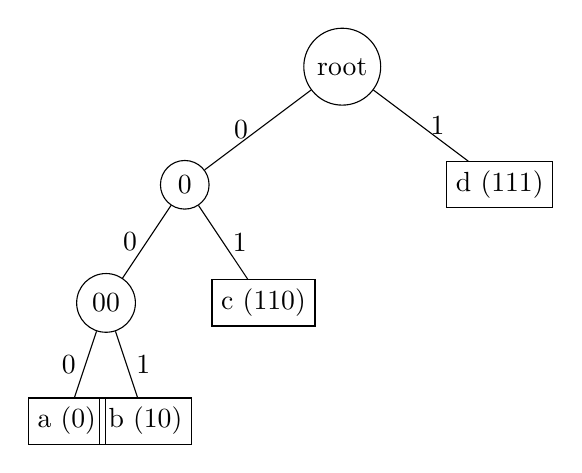
\begin{tikzpicture}[
    level distance=1.5cm,
    level 1/.style={sibling distance=4cm},
    level 2/.style={sibling distance=2cm},
    level 3/.style={sibling distance=1cm}
]
\node [circle, draw] {root}
    child {
        node [circle, draw] {0}
        child {
            node [circle, draw] {00}
            child {
                node [rectangle, draw] {a (0)}
                edge from parent node[left] {0}
            }
            child {
                node [rectangle, draw] {b (10)}
                edge from parent node[right] {1}
            }
            edge from parent node[left] {0}
        }
        child {
            node [rectangle, draw] {c (110)}
            edge from parent node[right] {1}
        }
        edge from parent node[left] {0}
    }
    child {
        node [rectangle, draw] {d (111)}
        edge from parent node[right] {1}
    };
\end{tikzpicture}
\caption{Binary tree representation of prefix code: a=0, b=10, c=110, d=111}
\end{figure}

\subsection{Optimal Code Lengths}
For a source with symbol probabilities $p_i$, optimal codeword lengths satisfy:
\[
\ell_i^* = \lceil -\log_2 p_i \rceil
\]
These satisfy Kraft inequality and are close to the theoretical minimum.

\begin{examplebox}
For symbols with probabilities $\{0.5, 0.25, 0.125, 0.125\}$:
\begin{align*}
\ell_1 &= \lceil -\log_2 0.5 \rceil = \lceil 1 \rceil = 1 \\
\ell_2 &= \lceil -\log_2 0.25 \rceil = \lceil 2 \rceil = 2 \\
\ell_3 &= \lceil -\log_2 0.125 \rceil = \lceil 3 \rceil = 3 \\
\ell_4 &= \lceil -\log_2 0.125 \rceil = \lceil 3 \rceil = 3
\end{align*}
Check Kraft: $2^{-1} + 2^{-2} + 2^{-3} + 2^{-3} = 0.5 + 0.25 + 0.125 + 0.125 = 1$
\end{examplebox}

\subsection{Code Efficiency and Redundancy}
\begin{definitionbox}
\textbf{Code Efficiency}:
\[
\eta = \frac{H(X)}{L} \times 100\%
\]
\textbf{Redundancy}:
\[
\rho = L - H(X) \quad \text{(bits/symbol)}
\]
\end{definitionbox}

\subsubsection{Upper Bound on Efficiency}
From Shannon's theorem:
\[
\frac{H(X)}{H(X)+1} \leq \eta \leq 1
\]

\begin{examplebox}
For a source with $H(X) = 2.3$ bits/symbol and code achieving $L = 2.5$ bits/symbol:
\[
\eta = \frac{2.3}{2.5} \times 100\% = 92\%
\]
\[
\rho = 2.5 - 2.3 = 0.2 \text{ bits/symbol}
\]
\end{examplebox}

\subsection{Extended Coding (Block Coding)}
By coding blocks of $n$ symbols together:
\begin{itemize}
    \item Achieve average length per symbol: $L_n/n \rightarrow H(X)$ as $n \rightarrow \infty$
    \item Redundancy per symbol: $\rho_n < 1/n$
    \item Trade-off: Larger $n$ requires more memory and complexity
\end{itemize}

\subsection{Proof Sketch of Shannon's Theorem}
\subsubsection{Lower Bound \texorpdfstring{($L \geq H(X)$)}{(L >= H(X))}}
\begin{enumerate}
    \item Let $p_i$ be symbol probabilities, $\ell_i$ be codeword lengths
    \item From information theory: $-\log_2 p_i$ is the ideal length
    \item Using Gibbs' inequality or convexity arguments:
    \[
    \sum p_i \ell_i \geq -\sum p_i \log_2 p_i = H(X)
    \]
\end{enumerate}

\subsubsection{Upper Bound \texorpdfstring{($L < H(X) + 1$)}{(L < H(X) + 1)}}
\begin{enumerate}
    \item Choose lengths: $\ell_i = \lceil -\log_2 p_i \rceil$
    \item Then: $-\log_2 p_i \leq \ell_i < -\log_2 p_i + 1$
    \item Multiply by $p_i$ and sum:
    \[
    H(X) \leq \sum p_i \ell_i < H(X) + 1
    \]
\end{enumerate}

\subsection{Applications and Implications}
\begin{importantbox}
\textbf{Practical Implications}:
\begin{itemize}
    \item Entropy provides the absolute limit for lossless compression
    \item Real compressors have additional overhead (model storage, headers)
    \item For small alphabets, the "+1" term can be significant
    \item Block coding helps approach the entropy limit
\end{itemize}
\end{importantbox}

\subsection{Limitations and Extensions}
\subsubsection{Assumptions in Shannon's Theorem}
\begin{itemize}
    \item Discrete memoryless source (symbols independent)
    \item Known probability distribution
    \item Noiseless channel
    \item These assumptions are often violated in practice
\end{itemize}

\subsubsection{Extensions}
\begin{itemize}
    \item \textbf{Markov sources}: Consider dependencies between symbols
    \item \textbf{Universal coding}: No prior knowledge of distribution
    \item \textbf{Rate-distortion theory}: Lossy compression extension
\end{itemize}

\subsection{Algorithm: Constructing a Prefix Code from Given Lengths}
\begin{algorithm}[H]  % Changed to [H]
\caption{Construct Prefix Code from Lengths}
\begin{algorithmic}[1]
\REQUIRE Codeword lengths $\ell_1, \ell_2, \ldots, \ell_n$ satisfying Kraft inequality
\ENSURE Prefix code with given lengths
\STATE Sort lengths in non-decreasing order: $\ell_{(1)} \leq \ell_{(2)} \leq \cdots \leq \ell_{(n)}$
\STATE Initialize current code to 0 (binary)
\FOR{$i = 1$ to $n$}
    \STATE Assign current code to symbol with length $\ell_{(i)}$
    \STATE Increment current code (binary addition)
    \STATE Shift left by $\ell_{(i+1)} - \ell_{(i)}$ bits (if $i < n$)
\ENDFOR
\RETURN The assigned codes
\end{algorithmic}
\end{algorithm}

\begin{examplebox}
Construct prefix code for lengths $\{2, 2, 3, 3\}$:
\begin{enumerate}
    \item Sorted lengths: $\{2, 2, 3, 3\}$
    \item Start with code = 00
    \item Assign: symbol1 = 00, increment → 01
    \item Assign: symbol2 = 01, increment → 10, no shift (same length)
    \item Assign: symbol3 = 10, increment → 11, shift left 1 bit → 110
    \item Assign: symbol4 = 110, done
\end{enumerate}
Result: $\{00, 01, 10, 110\}$
\end{examplebox}

\subsection{Homework Assignment}
\begin{enumerate}
    \item For a source with probabilities $\{0.4, 0.3, 0.2, 0.1\}$:
    \begin{itemize}
        \item Calculate the entropy
        \item Find optimal integer codeword lengths
        \item Verify they satisfy Kraft inequality
        \item Construct a prefix code with these lengths
        \item Calculate expected length and efficiency
    \end{itemize}

    \item Prove that for any prefix code with $n$ codewords, the average length satisfies:
    \[
    L \geq \log_2 n
    \]
    When does equality hold?

    \item Consider a binary source with $P(0) = p$. Plot:
    \begin{itemize}
        \item Entropy $H(p)$ vs $p$
        \item Minimum achievable $L$ vs $p$
        \item The gap $L - H(p)$ for simple coding schemes
    \end{itemize}

    \item Research and explain one practical limitation of Shannon's theorem in real-world compression systems.

    \item Design a prefix code for the alphabet $\{A, B, C, D, E, F\}$ with lengths $\{1, 2, 3, 3, 4, 4\}$. Show the binary tree representation.
\end{enumerate}

\subsection{Reading Assignment}
\begin{itemize}
    \item \textbf{Required}: Cover \& Thomas, Chapter 5: Data Compression
    \item \textbf{Required}: Sayood, Chapter 2: Mathematical Preliminaries
    \item \textbf{Recommended}: MacKay, Chapter 5: Symbol Codes
    \item \textbf{Additional}: Original papers by Shannon (1948) and Kraft (1949)
\end{itemize}

\subsection{Looking Ahead}
In the next lecture, we will explore:
\begin{itemize}
    \item Kolmogorov complexity: A different perspective on information
    \item Algorithmic information theory
    \item The concept of incompressibility
    \item Relationship between Kolmogorov complexity and practical compression
\end{itemize}

\end{document}
